\documentclass[10pt]{article}

% Idioma y codificación
\usepackage[utf8]{inputenc}
\usepackage[spanish]{babel}

% Márgenes
\usepackage{geometry}
\geometry{top=2.5cm, bottom=2.5cm, left=2.5cm, right=2.5cm}

% Gráficos y Tablas
\usepackage{pdflscape}
\usepackage{graphicx}
\usepackage{pdfpages}
\usepackage{multicol}
\usepackage{float}
\usepackage[table]{xcolor} % UNA SOLA VEZ Y CON [table]
\usepackage{booktabs}
\usepackage{xltabular}
\usepackage{caption}
\usepackage{subcaption}

% Listings para código
\usepackage{listings}
\lstdefinestyle{terminal}{
	backgroundcolor=\color{gray!10},
	basicstyle=\ttfamily\small,
	keywordstyle=\color{blue},
	commentstyle=\color{gray},
	frame=single,
	columns=fullflexible,
	morecomment=[l]{//}
}
\lstset{
	inputencoding=utf8,
	extendedchars=true,
	literate={á}{{\'a}}1 {é}{{\'e}}1 {í}{{\'i}}1 {ó}{{\'o}}1 {ú}{{\'u}}1 {ñ}{{\~n}}1
}

% Hipervínculos
\usepackage[hidelinks]{hyperref}
\hypersetup{
	colorlinks=true,
	linkcolor=blue,
	filecolor=magenta,
	urlcolor=cyan,
}

% Encabezados y pies de página
\usepackage{fancyhdr}
\pagestyle{fancy}
\fancyhf{}
\fancyfoot[R]{\thepage}

% Formato de títulos
\usepackage{titlesec}
\titleformat{\subsection}{\normalfont\large\bfseries}{\thesubsection}{1em}{}
\titleformat{\subsubsection}{\normalfont\normalsize\bfseries}{\thesubsubsection}{1em}{}

% Datos de la portada
\title{\textit{CARD PARTNER}\\ Una web para amantes de los \textit{TCGS}}

\author{
	\textbf{\small ÁLVAREZ FULCONIS, MARCOS PALATINO}\\
	\textbf{\small LÓPEZ PRIMO, ÁLVARO}\\
	\textbf{\small OTERO GARCÍA, SERGIO}\\
	\textbf{\small SANTIESTEBAN MENDO, EDGAR}
}

\date{Curso 25-26}

\begin{document}
	
	\begin{titlepage}
		\centering
		% Asegúrate de que la ruta al PDF de la UVA sea correcta
		%
\includegraphics[scale=0.3]{./Recursos/UVA-3881270087.pdf}\\[0.5cm] 
		\rule{\linewidth}{0.2mm}\\[0.4cm]
		{\huge\bfseries CARD PARTNER\par}
		{\large Una web para amantes de los TCGS\par}
		\rule{\linewidth}{0.2mm}\\[1.5cm]
		{\Large\bfseries Servicios y Sistemas Web}\\[0.3cm]
		{\large\bfseries Laboratorio L2 \\ GRUPO 33}\\[1cm]
		{\Large \begin{tabular}{c} ÁLVAREZ FULCONIS, MARCOS \\ LÓPEZ PRIMO, ÁLVARO \\ OTERO GARCÍA, SERGIO \\ SANTIESTEBAN MENDO, EDGAR \end{tabular}}\\[1.5cm]
		{\Large Curso 25-26}
	\end{titlepage}
	
	\pagenumbering{gobble}
	\tableofcontents \newpage
	
	\pagenumbering{arabic} 
	\setcounter{page}{1}
	
	\section{Base de datos}
		Para la base de datos se ha elegido usar MariaDB a través de XAMPP para facilitar el trabajo de gestión y diseño, ya que permite usar phpMyAdmin desde navegadores web y gestionar la base de datos de manera visual y exportar o importar los scripts de creación e inserción de datos,  además de otras herramientas útiles (como el meter csv)
		
		\subsection{Cambios del Modelo de Dominio a Entidad-Relacion}
			Para traducir el modelo de dominio realizado en la práctica 2 al modelo entidad-relacion de la base de datos, se han realizado los siguientes cambios:
			\begin{itemize}
				\item \textbf{Usuario}: \\
					Se ha traducido la relación de \textit{Usuario} como clase padre de \textit{Jugador} y \textit{Admin} a una sola tabla \texttt{Usuario} y un atributo ROL que especifique que tipo de usuario es.
				\item \textbf{Mazo}: \\
					Al igual que con \textit{Usuario}, la clase \textit{Mazo} se ha traducido a una única tabla \texttt{Mazo} y un atributo ES\_OFICIAL para hacer la distinción.
				\item \textbf{Relaciones *:*}: \\
					Las relaciones muchos a muchos entre \textit{Jugador}-\textbf{GUARDA}-\textit{Mazo}, \textit{Mazo}-\textbf{CONTIENE}-\textit{Carta} y \textit{Jugador}-\textbf{VALORA}-\textit{Mazo} se han traducido como las clases intermedias \texttt{GUARDA\_MAZO}, \texttt{CONTIENE\_CARTA} y \texttt{VALORACION} respectivamente.
				\item \textbf{}: \\
				
				
			\end{itemize}
			
			\begin{figure}[H]
				\centering
				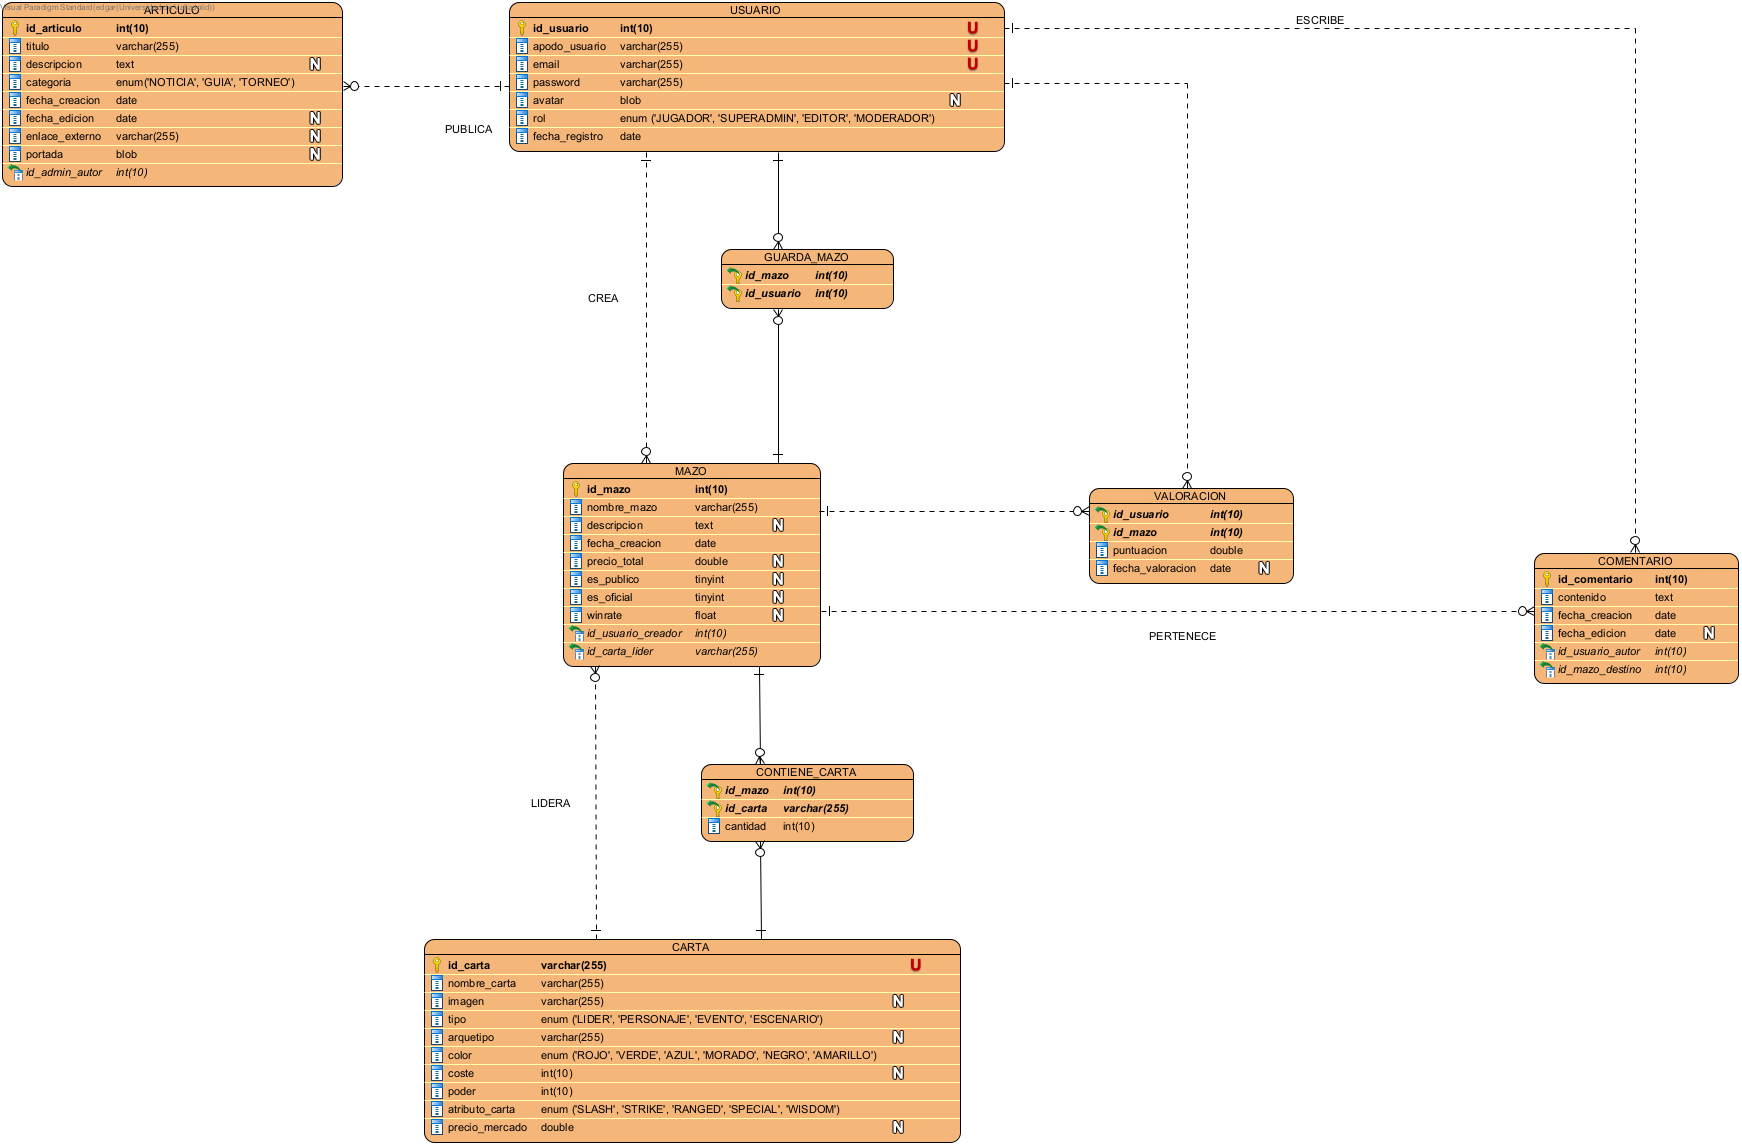
\includegraphics[width=1\textwidth]{Recursos/CardPartner_DB.png}
				\caption{Entidad-Relacion de la base de datos}
				\label{fig:mapa_sitio}
			\end{figure}
			
		\subsection{Estructura de la base de datos}
			
			Con el esquema entidad-relación realizado, el script de creación de la base de datos es:
			
			%Script creacion
			
			%Hablar de los tipos de datos que puedan ser llamativos y decisiones generales detras de nullable, timestamps vs date, defaults, etc
		
		\subsection{Inserción de datos}
			
	\newpage
	\section{Reparto de carga de trabajo}
	Todos los integrantes hemos participado en todas las fases del trabajo y repartido el trabajo de forma equitativa, aunque encargándonos cada uno especialmente de alguna parte.\\
	
	\begin{table}[h]
		\centering
		\caption{Distribución de Responsabilidades por Miembro}
		\begin{tabularx}{\textwidth}{llX} 
			\toprule
			\textbf{Nombre} & \textbf{Porcentaje} & \textbf{Responsabilidad principal} \\
			\midrule
			ÁLVAREZ FULCONIS, MARCOS PALATINO      	& 25\%                & Diseño de las vistas tcg, social,noticias,torneo y guías\\
			LOPEZ PRIMO, ÁLVARO      				& 25\%                & Diseño del index, login y todas sus opciones, creación del repositorio de github, redacción del documento\\
			OTERO GARCÍA, SERGIO     				& 25\%                & Diseño de decks y todos sus submenús, \textit{comunity decks, meta decks}, creación de mazos,vista de cartas\\
			SANTIESTEBAN MENDO, EDGAR    			& 25\%                & Modelo de dominio,flujos de navegación, requisitos y redacción del documento\\
			\bottomrule
		\end{tabularx}
	\end{table}
	
	
	\section{Declaración de Uso de Inteligencia Artificial}
	Para esta segunda entrega, se ha usado la IA Gemini como herramienta para dudas y mejoras del archivo LaTeX, revisión de los contenidos y evaluación de los mismos y diseño iterativo para mejorar lo ya realizado.\\
	Además, se ha usado \href{https://gemini.google.com/share/7a923a0bfae8}{Gemini} para la generación del logo del proyecto.
	
	\textbf{Ejemplos de prompts realizados:}
	\begin{itemize}
		\item 'Cómo podemos realizar un menú desplegable en html a partir de un botón'
		\item 'Cómo podemos hcer un enlace en una imagen'
		\item 'Cómo podemos hacer un popup para cambiar la contraseña'
		\item 'Cómo funciona un hover en html'
		\item 'Redimensionar los botones para que ocupen una parte proporcional del encabezado'
		\item 'En css por qué me sale un link subrayado'
		\item 'Como puedo hacer un popup con sobreado'
		\item 'La estructura de un proyecto html cuál es'
		\item 'Entre la idea X y la idea Y, dime posibles ventajas y desventajas de cada uno y cuál se adaptaría mejor al proyecto y por qué'
	\end{itemize}
	
	%\begin{itemize}
	%   \item Herramientas utilizadas: hay que especificar qué herramientas de IA se han utilizado.
	%  \item Propósito del uso: explicar cómo se ha utilizado cada herramienta.
	% \item Alcance del uso: indicar en qué partes específicas del trabajo se ha recibido asistencia de una herramienta de IA.
	%\item Prompts utilizados: incluir los prompts, preguntas o instrucciones exactas que se han
	%introducido en la herramienta de IA.
	%\end{itemize}
	
\end{document}